\subsection{Patchplot Library}
\label{sec:lib:patchplots}
\begin{pgfplotslibrary}{patchplots}
	A library for advanced |patch| plots. It has been designed to visualize shaded isoparametric finite element meshes of higher order. Its core is an interface to the generation of smoothly shaped elements with interpolated color values (based on \texttt{.pdf} Shading Type 6 and \texttt{.pdf} Shading Type 7), with additional (limited) support for constant color filling without shadings.

\subsubsection{Additional Patch Types}
\begin{pgfplotskey}{patch type=\mchoice{default,rectangle,triangle,line,bilinear,triangle quadr,biquadratic,coons} (initially default)}
	The |patchplots| library supports several new |patch type|s in addition to the initially available choices (which are |rectangle|,|triangle| and |line|). The documentation of these choices are replicated from page~\pageref{key:patch:type} here.

	The |patchplots| library is especially strong for |shader=interp|, so this is our main focus in the documentation here.

	\paragraph{Attention:} At the time of this writing, many free pdf viewers do not fully support the following shadings\footnote{The author of this package has submitted bugfixes to Linux viewers based on xpdf/libpoppler, so the problem will vanish in the future versions.}. The preferred viewer is Adobe Acrobat Reader.

	The choice \declaretext{rectangle} expects one or more rectangular patches with $n=4$ vertices each. These vertices are either encoded as a matrix or as individual patches (using |mesh input=patches|), in the sequence in which you would connect the vertices:
\begin{codeexample}[]
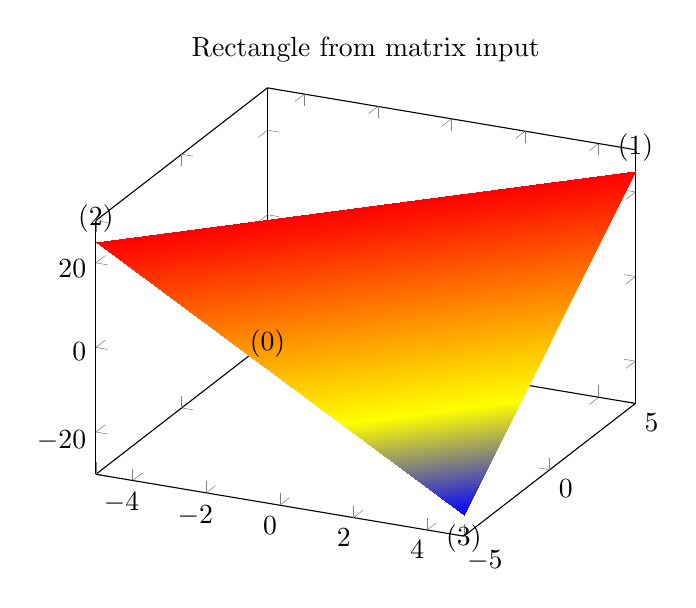
\begin{tikzpicture}
\begin{axis}[nodes near coords={(\coordindex)},
	title=Rectangle from matrix input]
% note that surf implies 'patch type=rectangle'
\addplot3[surf,shader=interp,samples=2,
	patch type=rectangle] 
	{x*y};
\end{axis}
\end{tikzpicture}
\end{codeexample}
\begin{codeexample}[]
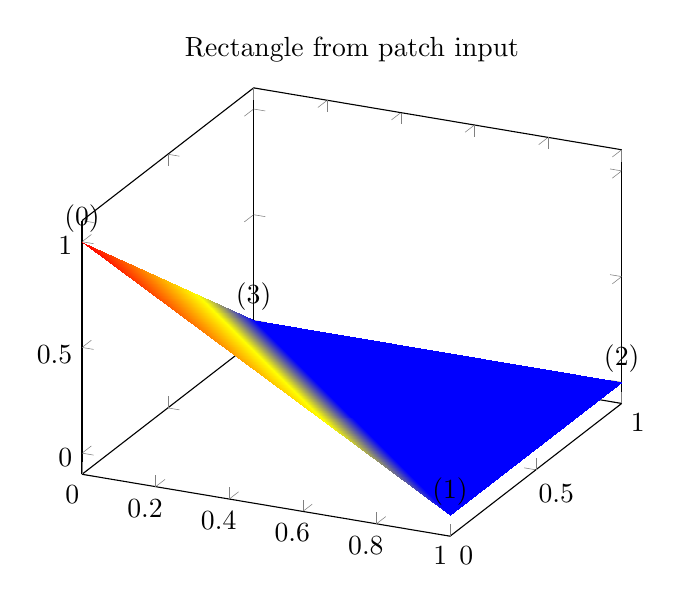
\begin{tikzpicture}
\begin{axis}[nodes near coords={(\coordindex)},
	title=Rectangle from patch input]
\addplot3[patch,shader=interp,patch type=rectangle] coordinates {
	(0,0,1) (1,0,0) (1,1,0) (0,1,0)
};
\end{axis}
\end{tikzpicture}
\end{codeexample}
	\noindent As already documented on page~\pageref{key:patch:type}, the |shader=interp| implementation for |rectangle| uses two triangles and interpolates them linearly.

	The choice \declareandlabel{bilinear} is essentially the same as |rectangular| with respect to its input formats and stroke paths, but it uses correct bilinear shading for |shader=interp|. The two examples from above now become
\begin{codeexample}[]
\begin{tikzpicture}
\begin{axis}[nodes near coords={(\coordindex)},
	title=Bilinear from $2\times 2$ matrix input]
% note that surf implies 'patch type=rectangle'
\addplot3[surf,shader=interp,samples=2,
	patch type=bilinear] 
	{x*y};
\end{axis}
\end{tikzpicture}
\end{codeexample}
\begin{codeexample}[]
\begin{tikzpicture}
\begin{axis}[nodes near coords={(\coordindex)},
	title=Bilinear from $4$--point patch input]
\addplot3[patch,shader=interp,patch type=bilinear] coordinates {
	(0,0,1) (1,0,0) (1,1,0) (0,1,0)
};
\end{axis}
\end{tikzpicture}
\end{codeexample}

	The choice \declaretext{triangle} expects a sequence of linear triangles, each encoded using $n=3$ vertices:
\begin{codeexample}[]
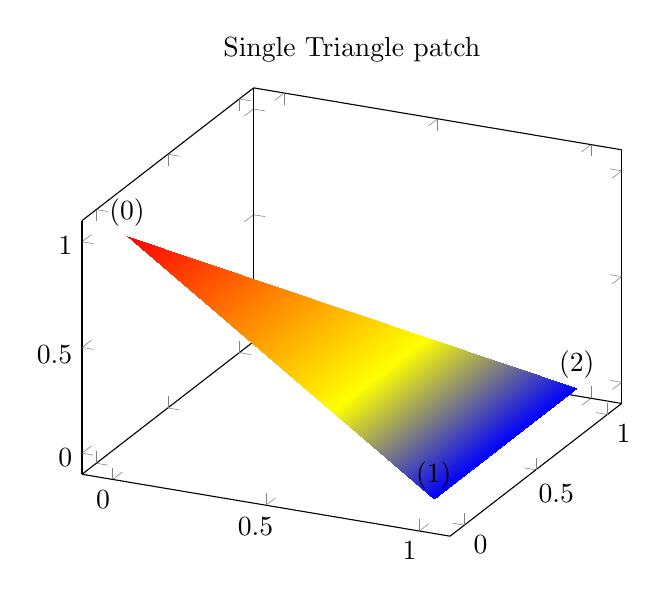
\begin{tikzpicture}
\begin{axis}[enlargelimits,
	nodes near coords={(\coordindex)},
	title=Single Triangle patch]
\addplot3[patch,shader=interp] coordinates {
	(0,0,1)
	(1,0,0)
	(1,1,0)
};
\end{axis}
\end{tikzpicture}
\end{codeexample}

	The choice \declareandlabel{triangle quadr} expects a sequence of isoparametric quadratic triangles, each defined by $n=6$ vertices:
\begin{codeexample}[]
\begin{tikzpicture}
\begin{axis}[nodes near coords={(\coordindex)},
	title=Quadratic Triangle]
\addplot[patch,patch type=triangle quadr,
	shader=interp,point meta=explicit]
coordinates {
	(0,0) [1] (5,4) [2] (0,7) [3]
	(2,3) [1] (3,6) [2] (-1,4)  [3]
};
\end{axis}
\end{tikzpicture}
\end{codeexample}
\begin{codeexample}[]
\begin{tikzpicture}
\begin{axis}[nodes near coords={(\coordindex)},
	title=Quadratic Triangle]
\addplot3[patch,patch type=triangle quadr,
	shader=interp]
coordinates {
	(0,0,1) (5,4,0) (0,7,0)
	(2,3,0) (3,6,0) (-1,4,0)
};
\end{axis}
\end{tikzpicture}
\end{codeexample}
	\noindent Here, the edges have the correct quadratic shape. However, the color interpolation is just \emph{bilinear}; using the color values of the corners and ignoring the rest (consider using |patch refines| to improve the color interpolation). For three dimensions, \PGFPlots\ checks the depth of corners to determine foreground/background. For two dimensions, strongly distorted elements may fold over each other in unexpected ways. 

	The choice \declareandlabel{biquadratic} expects a sequence of isoparametric biquadratic quadrilaterals (rectangles), each defined by $n=9$ vertices:
\begin{codeexample}[]
\begin{tikzpicture}
\begin{axis}[nodes near coords={(\coordindex)},
	title=Single Biquadratic Quadrilateral]
\addplot[patch,patch type=biquadratic,
	shader=interp,point meta=explicit]
coordinates {
	(0,0) [1] (6,1) [2] (5,5) [3] (-1,5) [4]
	(3,1) [1] (6,3) [2] (2,6) [3] (0,3) [4]
	(3,3.75) [4]
};
\end{axis}
\end{tikzpicture}
\end{codeexample}
\begin{codeexample}[]
\begin{tikzpicture}
\begin{axis}[nodes near coords={(\coordindex)},
	title=Single Biquadratic Quadrilateral]
\addplot3[patch,patch type=biquadratic,shader=interp]
coordinates {
	(0,0,1) (6,1,0) (5,5,0) (-1,5,0)
	(3,1,0) (6,3,0) (2,6,0) (0,3,0)
	(3,3.75,0)
};
\end{axis}
\end{tikzpicture}
\end{codeexample}
	\noindent Similar to |triangle quadr|, the edges have the correct quadratic shape -- but the color interpolation is just \emph{bilinear}; using the color values of the corners and ignoring the rest. Again, consider using |patch refines| to improve the color interpolation.

	The choice \declareandlabel{coons} expects a sequence of one or more coons patches, made up of $n=12$ points each. A coons patch is delimited by four cubic Bezier curves, with the end points attached to each other -- and the $n$ points provide the required control points for these curves in a specific ordering which is illustrated in the following example:
\begin{codeexample}[]
\begin{tikzpicture}
\begin{axis}[nodes near coords={(\coordindex)},
	width=12cm,
	title=A Coons Patch]
\addplot[mark=*,patch,patch type=coons,
	shader=interp,point meta=explicit] 
coordinates {
	(0,0)   [0] % first corner
	(1,-1)  [0] % bezier control point between (0) and (3)
	(4,0.7) [0] % bezier control point between (0) and (3)
	%
	(3,2)   [1] % second corner
	(4,3.5) [1] % bezier control point between (3) and (6)
	(7,2)   [1] % bezier control point between (3) and (6)
	%
	(7,1)      [2] % third corner
	(6,0.6)    [2] % bezier control point between (6) and (9)
	(4.5,-0.5) [2] % bezier control point between (6) and (9)
	%
	(5,-2)   [3] % fourth corner
	(4,-2.5) [3] % bezier control point between (9) and (0)
	(-1,-2)  [3] % bezier control point between (9) and (0)
};
\end{axis}
\end{tikzpicture}
\end{codeexample}
	\noindent The four cubic Bezier curves are \emph{equivalent} to \texttt{curveto} paths of \pgfname, i.e.\  \parg{corner 1}|.. controls|\parg{control point A}| and |\parg{control point B}| .. |\parg{corner 2} paths. The interpolated shading is bilinear. More precisely, a bilinear shading in the unit cube $[0,1]^2$ is initialised which is then mapped into the coons patch such that the corners match. The color interpolation uses only the color data of the four corners, color values of intermediate control points are ignored for the shading (although their value will be respected for the upper and lower limit of color data). In contrast to the finite element patches, a coons patch is inherently two--dimensional. While you can still use three--dimensional coordinates, \PGFPlots\ will draw the shading as you provide it, without checkout for the depth information (as it does for the other |patch type|s). In other words: depending on the current |view| angle, the shading might fold over itself in unexpected ways.

	Even for two dimensions, coons patches may fold over themselves. To determine which part is foreground and which part is background, the following rule applies: the four corner points $(0)$, $(3)$, $(6)$, $(9)$ are associated to the unit cube points $(u,v) = (0,0)$, $(0,1)$, $(1,1)$ and $(1,0)$, respectively. The edge between corner $(3)$ and $(6)$ (i.e. the one with $v=1$) is foreground, the edge between $(1)$ and $(9)$ is background. Thus, large values of $v$ are drawn on top of small values of $v$. If $v$ is constant, large values of $u$ are drawn on top of small values of $u$. Thus, reordering the patch vertices (choosing a different first vertex and/or reversing the sequence) allows to get different foreground/background configurations\footnote{Internally, \PGFPlots\ employs such mechanisms to map the higher order isoparametric patch types to coons patches, sorting according their corner's depth information.}.
	
\end{pgfplotskey}

\subsubsection{Automatic Patch Refinement and Triangulation}

\begin{pgfplotskey}{patch refines=\marg{integer} (initially 0)}
	
\end{pgfplotskey}

\begin{pgfplotskey}{patch to triangles=\mchoice{true,false} (initially false)}
	
\end{pgfplotskey}

\end{pgfplotslibrary}
